%% 
%% ACS project dissertation template. 
%% 
%% Currently designed for printing two-sided, but if you prefer to 
%% print single-sided just remove ",twoside,openright" from the 
%% \documentclass[] line below. 
%%
%%
%%   SMH, May 2010. 


\documentclass[a4paper,12pt,twoside,openright]{report}


%%
%% EDIT THE BELOW TO CUSTOMIZE
%%

\def\authorname{David Brazdil\xspace}
\def\authorcollege{Trinity Hall\xspace}
%\def\authoremail{Sarah.Jones@cl.cam.ac.uk}
\def\dissertationtitle{Java Native Interface on CHERI}
\def\wordcount{14,235}


\usepackage{epsfig,graphicx,parskip,setspace,tabularx,xspace,url} 

%% START OF DOCUMENT
\begin{document}


%% FRONTMATTER (TITLE PAGE, DECLARATION, ABSTRACT, ETC) 
\pagestyle{empty}
\singlespacing
% title page information
\begin{titlepage} 

\begin{center}
\noindent
\huge
\dissertationtitle \\
\vspace*{\stretch{1}}
\end{center}

\begin{center}
\noindent
\huge
\authorname \\
\Large
Computer Science Tripos, Part III \\
\authorcollege      \\[24pt]

\includegraphics{CUni3.eps}
\end{center}

\vspace{24pt} 

\begin{center}
\noindent
\large

\vspace*{\stretch{1}}
\end{center}

\begin{center}
\noindent
University of Cambridge \\
Computer Laboratory     \\
William Gates Building  \\
15 JJ Thomson Avenue    \\
Cambridge CB3 0FD       \\
{\sc United Kingdom}    \\
\end{center}

%\begin{center}
%\noindent
%Email: \authoremail \\
%\end{center}

\begin{center}
\noindent
\today
\end{center}

\end{titlepage} 

\newpage
\vspace*{\fill}

\onehalfspacing
\newpage
{\Huge \bf Declaration}

\vspace{24pt} 

I \authorname of \authorcollege, being a candidate for the M.Phil in
Advanced Computer Science, hereby declare that this report and the
work described in it are my own work, unaided except as may be
specified below, and that the report does not contain material that
has already been used to any substantial extent for a comparable
purpose.

\vspace{24pt}
Total word count: \wordcount

\vspace{60pt}
\textbf{Signed}: 

\vspace{12pt}
\textbf{Date}:


\vfill

This dissertation is copyright \copyright 2010 \authorname. 
\\
All trademarks used in this dissertation are hereby acknowledged.



\newpage
\vspace*{\fill}

\singlespacing
\newpage
{\Huge \bf Abstract}
\vspace{24pt} 

With the necessity to reuse legacy code, or to employ readily available third-party libraries, it is not uncommon for large applications to be written in more than one programming language. Such heterogeneous environments have inherent advantages, e.g.\ allowing security-critical components to be written in a memory-safe language like Java, while performance-critical code in C, but because there is no runtime separation between the two code bases, it is possible for the native code to corrupt the Java environment or to bypass its security.

Qishr demonstrates that the capability-enabled CHERI processor can be used to isolate Java native code into a safe sandbox, from which it can only interact with the Java runtime and the system kernel through a secure interface. It guarantees that the code cannot break memory safety of Java objects, controls its access to system resources in accordance with the security policy enforced by Java on its classes, and provides a compatibility layer for legacy code written against the standard native interface.

\newpage
\vspace*{\fill}


\pagenumbering{roman}
\setcounter{page}{0}
\pagestyle{plain}
\tableofcontents
\listoffigures
\listoftables

\onehalfspacing

%% START OF MAIN TEXT 

\chapter{Introduction}
\pagenumbering{arabic} 
\setcounter{page}{1} 

% This is the introduction where you should introduce your work.  In
% general the thing to aim for here is to describe a little bit of the
% context for your work --- why did you do it (motivation), what was the
% hoped-for outcome (aims) --- as well as trying to give a brief
% overview of what you actually did.
% 
% It's often useful to bring forward some ``highlights'' into 
% this chapter (e.g.\ some particularly compelling results, or 
% a particularly interesting finding). 
% 
% It's also traditional to give an outline of the rest of the
% document, although without care this can appear formulaic 
% and tedious. Your call. 



\begin{enumerate}
	\item Java applications need 
\end{enumerate}

\chapter{Background} 

% A more extensive coverage of what's required to understand your 
% work. In general you should assume the reader has a good undergraduate 
% degree in computer science, but is not necessarily an expert in 
% the particular area you've been working on. Hence this chapter 
% may need to summarize some ``text book'' material. 
% 
% This is not something you'd normally require in an academic paper, 
% and it may not be appropriate for your particular circumstances. 
% Indeed, in some cases it's possible to cover all of the ``background'' 
% material either in the introduction or at appropriate places in 
% the rest of the dissertation. 

\section{Java Security Architecture}

Java was designed mainly as a universal platform for networked environments which necessarily made its security model one of the most important architectural features. On all its levels, Java addresses the common pitfalls of modern software engineering which can lead to introduction of security vulnerabilities, and thus guarantees a minimal level of application robustness and alleviates the process of implementing additional security measures.

At the core of the platform lies the Java programming language, an easy-to-learn type-safe language with automatic memory management and built around the principles of object-oriented programming. These properties significantly reduce the likelihood of writing unsafe code and also encourage the principle of least privilege via separation of executable code and its state into smaller object-level protection domains.

Java applications are expected to be distributed over public networks and therefore the platform has to account for composition of code with varying level of trust. Untrusted code can be executed inside a safe environment isolated from other code running inside the same virtual machine and be subject to a programmatically managed security policy which can limit its access to guarded resources.

Additionally, the Java framework provides a large set of extensible security APIs with ready-to-use implementation of many cryptographic algorithms and standardized protocols for public key infrastructure, authorization and encrypted network communication. 

\subsection{Code Safety}

The security of the Java platform is deeply rooted in the type, memory and control flow safety properties of its executable code. The language and the instruction set were crafted in a way that program bugs are likely to be caught by the compiler and pre-execution bytecode verifier, and other will raise an exception at runtime. 

Java's type system is primarily dynamic, although most types are actually checked statically for the sake of performance. Operations which are checked at runtime include array assignments, operations on generic classes and type casts. Unfortunately, the type inference algorithm has been shown to contain vulnerabilities~\cite{Suenaga:2012:JavaVulnerability} which make way to type confusion attacks~\cite{Oh:2012:JavaExploitReport} and these can subsequently be exploited to bypasss the security of the entire platform~\cite{McGraw:1999:SJG:298616}.

Memory safety in Java is strongly connected to the principles of OOP. Code does not have direct access to the heap but rather has to adhere to a model of a memory space structured into object instances and their internal fields protected by the reference monitor, accessed through opaque references and automatically managed by the garbage collector. Together with the type system and explicit range checks, Java prevents common bugs which can give the attacker access to an arbitrary part of the memory, such as buffer overflow or dangling pointers.



\subsection{Policy enforcement}
reference monitor...

\subsection{Java Native Interface}

allows for type confusion

\begin{figure}
	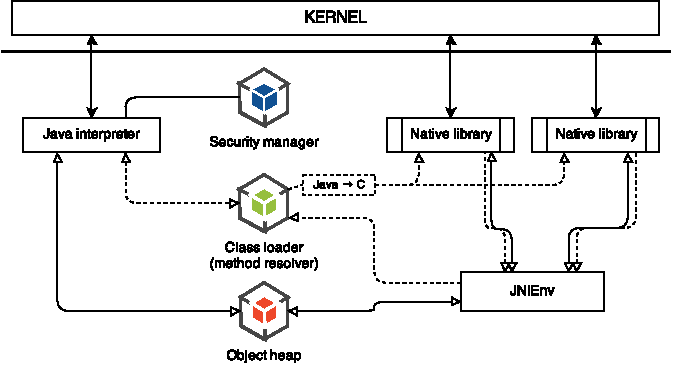
\includegraphics[width=\textwidth]{dia_jni_orig.pdf}
	\caption{Schematic diagram of the core JVM components in terms of security.}
\end{figure}

\section{Capability Hardware Enhanced RISC Instructions (CHERI)}

\section{Early capability systems}

\subsection{Hybrid capability architecture}

\subsection{Capability coprocessor}

\chapter{Related Work} 

This chapter covers relevant (and typically, recent) research 
which you build upon (or improve upon). There are two complementary 
goals for this chapter: 
\begin{enumerate} 
  \item to show that you know and understand the state of the art; and 
  \item to put your work in context
\end{enumerate} 

Ideally you can tackle both together by providing a critique of
related work, and describing what is insufficient (and how you do
better!)

The related work chapter should usually come either near the front or
near the back of the dissertation. The advantage of the former is that
you get to build the argument for why your work is important before
presenting your solution(s) in later chapters; the advantage of the
latter is that don't have to forward reference to your solution too
much. The correct choice will depend on what you're writing up, and
your own personal preference.

\section{Joe-E}

\section{Dalvik}

sandbox by linux uid

\section{SafeJNI}

section{Robusta}

doesn't support dynamic loading (and by design cannot)

\section{Capsicum}

\chapter{Design and Implementation} 

This chapter may be called something else\ldots but in general 
the idea is that you have one (or a few) ``meat'' chapters which
describe the work you did in technical detail. 

\section{Overview}

\subsection{Toolchain}

\section{Sandboxing}

\subsection{Security domains}

\section{Enforcing memory safety}

\section{Applying security policy}

all Java domains - language safety, security policies

VM domain remains the only one that can do system calls => GNU Classpath now provides services around system calls but those must go through the trusted trampoline

\section{Revoking access}

\chapter{Evaluation} 

For any practical projects, you should almost certainly have
some kind of evaluation, and it's often useful to separate 
this out into its own chapter. 


\chapter{Summary and Conclusions} 

As you might imagine: summarizes the dissertation, and draws 
any conclusions. Depending on the length of your work, and 
how well you write, you may not need a summary here. 

You will generally want to draw some conclusions, and point
to potential future work. 




\appendix
\singlespacing

\bibliographystyle{unsrt} 
\bibliography{acs-dissertation} 

\end{document}
